\documentclass[utf8,compress]{beamer}

\usetheme{Warsaw}
\usecolortheme{whale}

\usepackage[francais]{babel}
%tableofcontent with 2 cols
\usepackage{multicol}
%
\usepackage{textcomp}
%hide the warsaw default menu bar
\setbeamertemplate{headline}{}

%\newcommand{\slidesubject}{Présentation en \LaTeX}

\title{Développement de services Web JAX-RS pour l'import de données voirie et transport en commun}
\subtitle{\slidesubject{}}
%	\subject{\slidesubject{}}
\author{Bertrand \textsc{Guerrero}}
\institute{
    Formation professionnelle Concepteur / Développeur \\
    MobiGIS\\
    \vspace{0.8em}
    \emph{- Responsables -} \\
    M.~Christophe \textsc{Lapierre}\\
    M.~Julien \textsc{Lesbegueries}
}
\date{17 Juillet 2015}

%% Définition du répertoire contenant les images
\graphicspath{{images/}}

\logo{
\includegraphics[height=1cm]{logos_mobigis.jpg}}

%% Numérotation des slides :
%% http://texblog.net/latex-archive/plaintex/beamer-footline-frame-number/

%% Solution 1
%\newcommand*\oldmacro{}%
%\let\oldmacro\insertshorttitle%
%\renewcommand*\insertshorttitle{%
%  \oldmacro\hfill%
%  \insertframenumber\,/\,\inserttotalframenumber}

%% Solution 2
\expandafter\def\expandafter\insertshorttitle\expandafter{%
  %\insertshorttitle\hfill%
  \insertframenumber}

\begin{document}

\begin{frame}
\titlepage
\end{frame}

\logo{
\includegraphics[height=1cm]{logos_mobigis.jpg}}

\section{Plan}

\begin{frame}{Plan}
   \begin{multicols}{2}
	\tableofcontents
   \end{multicols}
\end{frame}

%% Un rappel du plan sera affiché à chaque début de section.
\AtBeginSection[]
{
  \begin{frame}<beamer>
    %\frametitle{Plan}
   \begin{multicols}{2}
     \tableofcontents[currentsection,hideothersubsection]
   \end{multicols}
  \end{frame}
}
\section{Présentation de l’entreprise}
\subsection{Entreprise MobiGIS}
\begin{frame}{Entreprise MobiGIS}
\begin{block}{Présentation}
Société de services en géomatique, et NTIC.\\	
L’activité de MobiGIS est centrée sur les services SIG et l’édition de logiciels. \\
\end{block}
\end{frame}
\begin{frame}{Services MobiGIS}
\begin{figure}[h]
    \center
    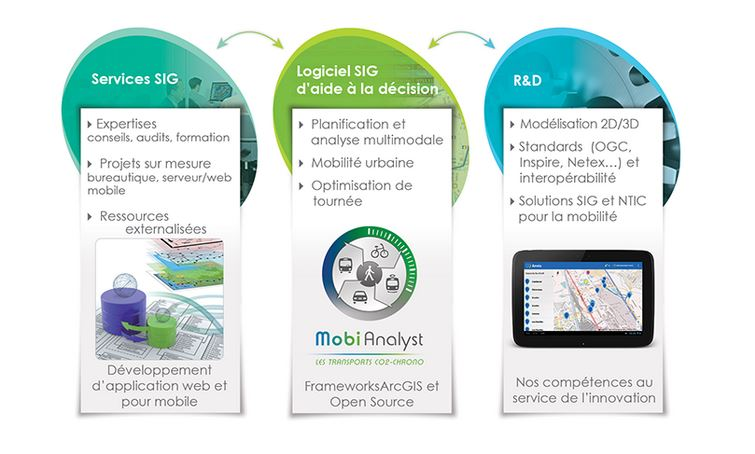
\includegraphics[width=\textwidth]{images/fig1_solutionsMobigis.JPG}
\end{figure}
\end{frame}
\begin{frame}{Activités de MobiGIS}
\begin{block}{Activités}
Les clients de MobiGIS sont par exemples des industries, la grande distribution, les collectivités locales, et
les intégrateurs et société de services en ingénierie informatique (SSII). \\
Les logiciels développés permettent de faire des analyses multiples : territoire, pollutions, démographie, etc., d'élaborer des plans de déplacement urbain et entreprise, d'étudier et de préparer la réorganisation des réseaux multimodaux et la création de nouvelles infrastructures de transport.
\end{block}
\end{frame}
\begin{frame}{Clients MobiGIS}
\begin{figure}[h]
    \center
    
\includegraphics[width=\textwidth]{images/fig2_referencesMobigis.JPG}
\end{figure}
\end{frame}
\subsection{Domaine d'application}
\begin{frame}{Domaine d'application}
\begin{block}{Les Systèmes d’Informations Géographiques (SIG)}
Les Systèmes d’Informations Géographiques (SIG) sont des outils informatiques permettant
de représenter et d’analyser toutes les choses qui existent sur terre ainsi que tous les événements
qui s’y produisent. \\
Le SIG appliqué aux transports, peut être utilisé
pour gérer et analyser certaines informations essentielles :\\
— Planification et modélisation des transports\\
— Planification et analyse des itinéraires\\
— Localisation et suivi automatiques des véhicules\\
\end{block}
\end{frame}
\subsection{Technologies}
\begin{frame}{Technologies}
\begin{block}{Compétences des équipes}
TECHNOLOGIES
\begin{itemize}
\item \textbf{Applications Web :} HTML5, CSS, Php, JavaScript, JQuery, Leaflet, Angular, API JavaScript, FLEX, OpenLayers
\item \textbf{Applications Mobiles :} Apache Cordova, PhoneGap, Android, iOS, Windows Phone
\item \textbf{Développement :} Java EE, C/C++, C\#, Python
\item \textbf{SIG :} ESRI (ArcObjects, ArcGIS, ArcGIS Server, Arcpy) GeoServer, PostGIS, QGIS, OpenLayers, Mapinfo, Google Maps
\item \textbf{Bases de données :} Oracle, SQL Server, PostgreSQL/PostGIS, MySQL, ArcSDE, SQLite
\item \textbf{Systèmes d’exploitation :} Windows Server – Linux – UNIX – iOS – Android
\end{itemize}
\end{block}
\end{frame}

\AtBeginSection[]
{
  \begin{frame}<beamer>
		\begin{multicols}{2}
     \tableofcontents[currentsection,hideothersubsection]
   \end{multicols}
  \end{frame}
}

\section{Contexte du stage}
\subsection{Projet MobiSAAS}
\begin{frame}{Projet MobiSAAS}
\begin{block}{Présentation}
Le projet \og MobiSAAS \fg : MobiAnalyst as a Service, s'inscrit dans la démarche d'entreprise de proposer des solutions en mode SAAS. Le projet consiste d'une manière générale à exposer les fonctionnalités de la solution Desktop du produit \og MobiAnalyst \fg
\end{block}
\end{frame}
\begin{frame}{Projet MobiSAAS}
\begin{block}{Interface (IHM) MobiSAAS}
\begin{figure}[h]
    \center
    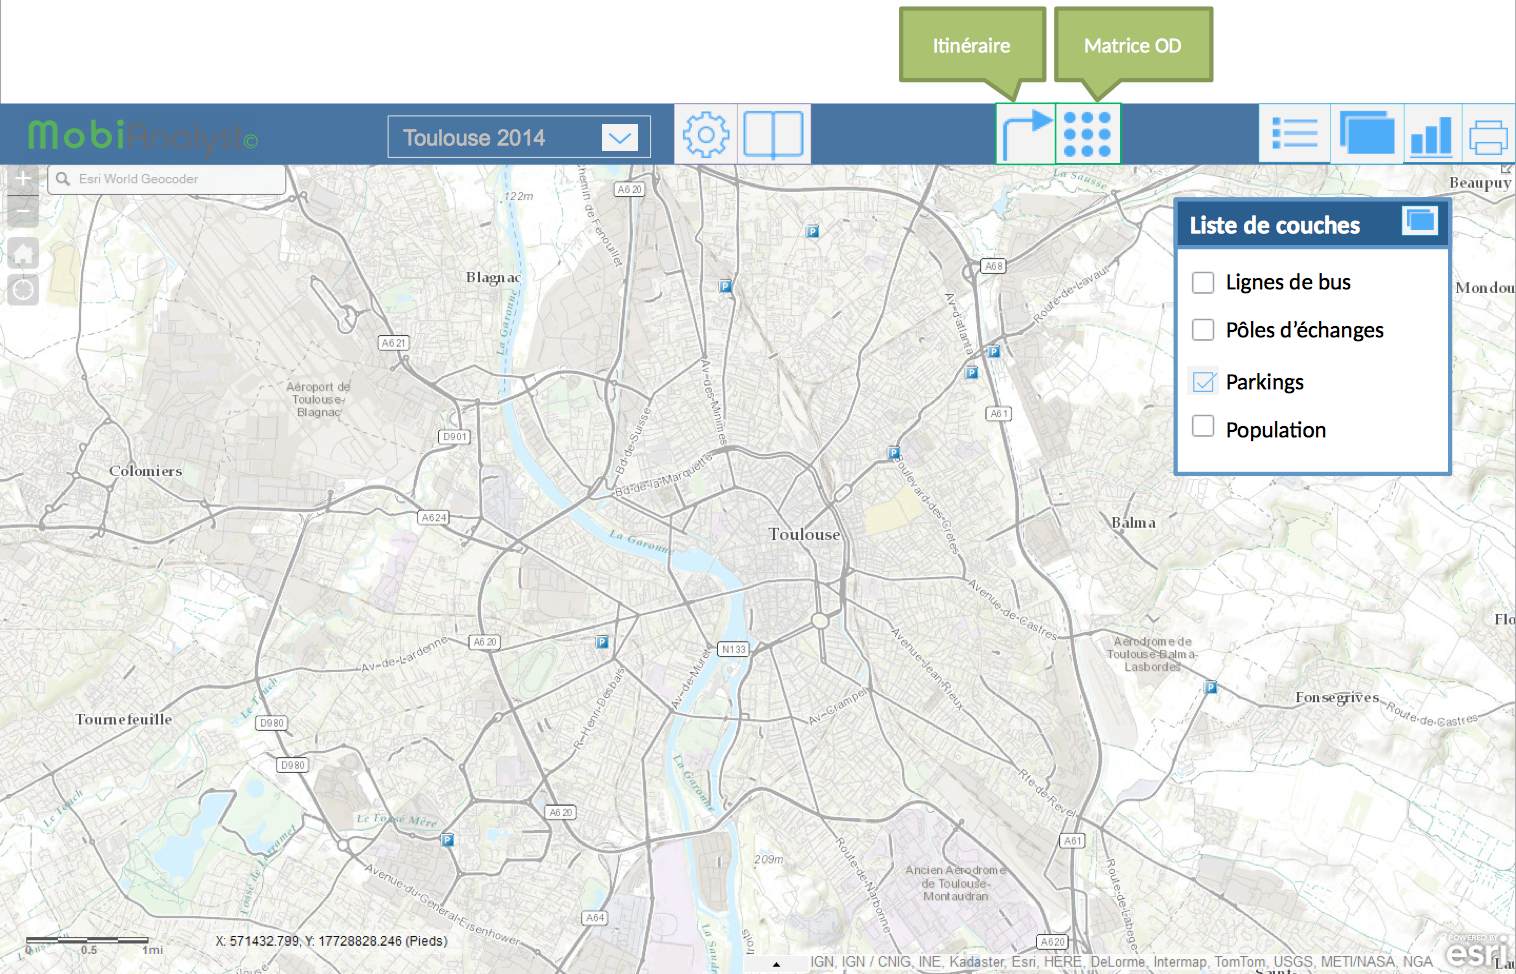
\includegraphics[width=\textwidth]{images/MobiSAAS_IHM.png}
\end{figure}
\end{block}
\end{frame}
\begin{frame}{Projet MobiSAAS}
\begin{block}{Objectifs du stage}
L'objectif du stage est le développement de web services permettant d'exposer des fonctionnalités d'importation de données voirie et transport en commun, pour la construction automatique de réseaux de transports multi-modaux
\end{block}
\begin{block}{API REST ?}
REST est un style d'architecture qui repose sur le protocole HTTP : On accède à une ressource (par son URI unique) pour procéder à diverses opérations (GET lecture / POST écriture / PUT modification / DELETE suppression), opérations supportées nativement par HTTP.
\end{block}
\end{frame}

\subsection{Cahier des charges}
\begin{frame}{Cahier des charges : Architecture}
\begin{block}{Architecture globale du module \og MobiAdmin \fg{} }
\begin{figure}[h]
    \center
    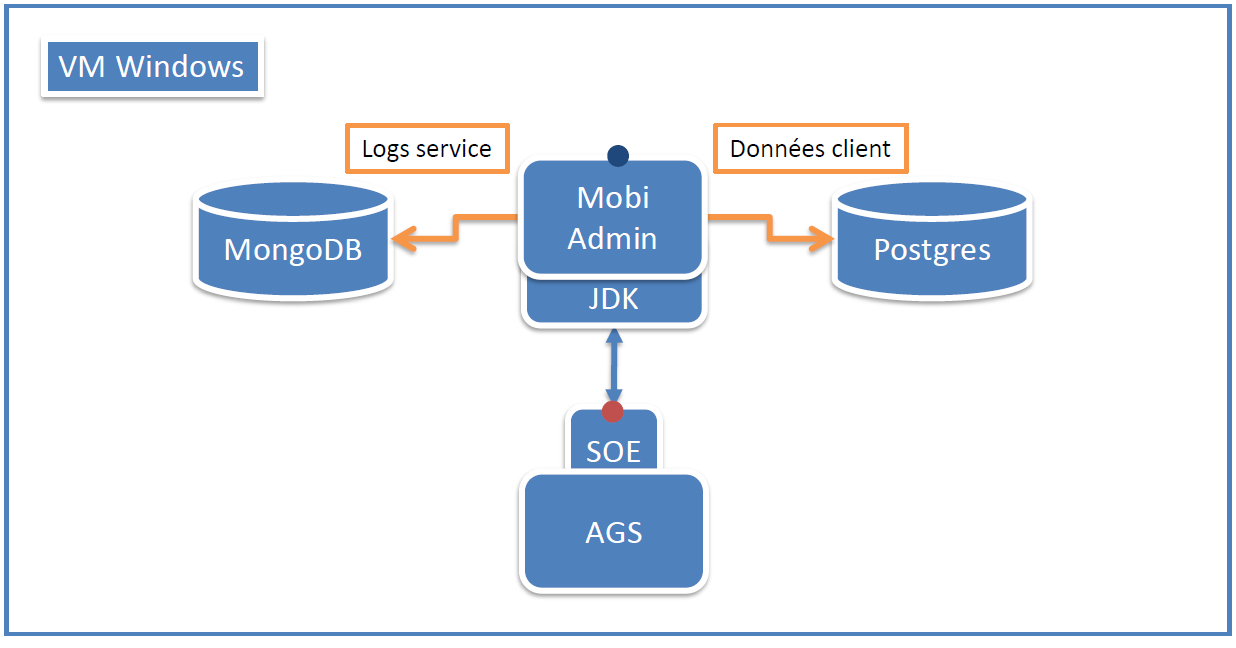
\includegraphics[width=\textwidth]{images/architecture.png}
\end{figure}
\end{block}
\end{frame}
\begin{frame}{Cahier des charges : Spécifications fonctionnelles}
\begin{block}{Les besoins}
Mon stage et les développements demandés concernent le composant d'administration de l'infrastructure : \og MobiAdmin \fg. \\

Dans l'objectif de gérer les données du client, je dois proposer un web service pour la gestion des données de transport dans l'espace privatif du client. La fonctionnalité principale à développer est donc un web service d'upload de données et plus particulièrement l'upload de données de transport public au format GTFS.
\end{block}
\end{frame}
\begin{frame}{Cahier des charges : Spécifications fonctionnelles}
\begin{block}{Composant \og MobiAdmin \fg{} }
\begin{figure}[h]
    \center
    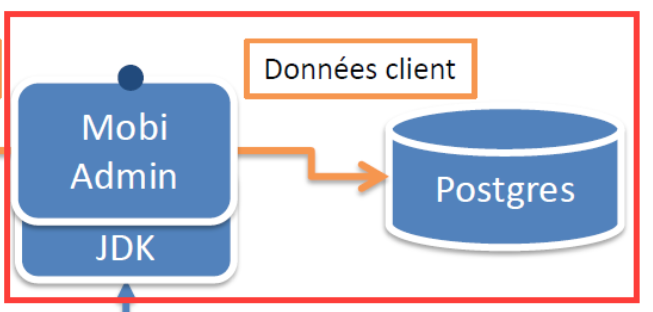
\includegraphics[width=\textwidth]{images/archi_module_admin.png}
\end{figure}
\end{block}
\end{frame}
\begin{frame}{Cahier des charges : Spécifications fonctionnelles}
\begin{block}{Les données clients}
Chaque upload est identifié par un UUID dans un répertoire client (ex: Tisseo)
Chaque upload est daté, et possède une \og trace \fg  dans la base postgres : \\
\item chemin vers la données, \\
\item statut de l'opération,\\
\item etc.
\end{block}
\end{frame}
\begin{frame}{Cahier des charges : Spécifications fonctionnelles}
\begin{block}{Les données GTFS}
Les données GTFS sont dans un archive (fichier au format .zip), qu'il faut extraire.
Un ou plusieurs jeu de données peuvent y être inclus.
Un jeu de données est composé d'au moins 8 fichiers (au format .txt).
\end{block}
\begin{block}{Un Web Service dédié GTFS}
L'objectif de ce web service est de stocker ces données, de récupérer des métadonnées. 
Par exemple : l'extension géographique des données, le nom de l'agence, le nombre de lignes, le mode de transport, etc.\\
Le service valide les jeux de données uploadés et produit un rapport de validation.\\
L'étape suivante consistera à charger ces données (.txt) dans la base postgres.
\end{block}
\end{frame}
\begin{frame}{Cahier des charges : Spécifications techniques}
\begin{block}{Spécifications techniques}
Pour le composant \og MobiAdmin \fg  (serveur REST) qui va héberger les services : utilisation du framework \textbf{Dropwizard} :\\
\begin{itemize}
\item orienté micro-services 
\item serveur HTTP « Jetty »
\item framework open source Jersey (spécification JAX-RS)
\item librairie Jackson 
\item etc.
\end{itemize}
\end{block}
\end{frame}
\begin{frame}{Cahier des charges : Application multi-couches}
\begin{block}{Application multi-couches}
\begin{figure}[h]
    \center
    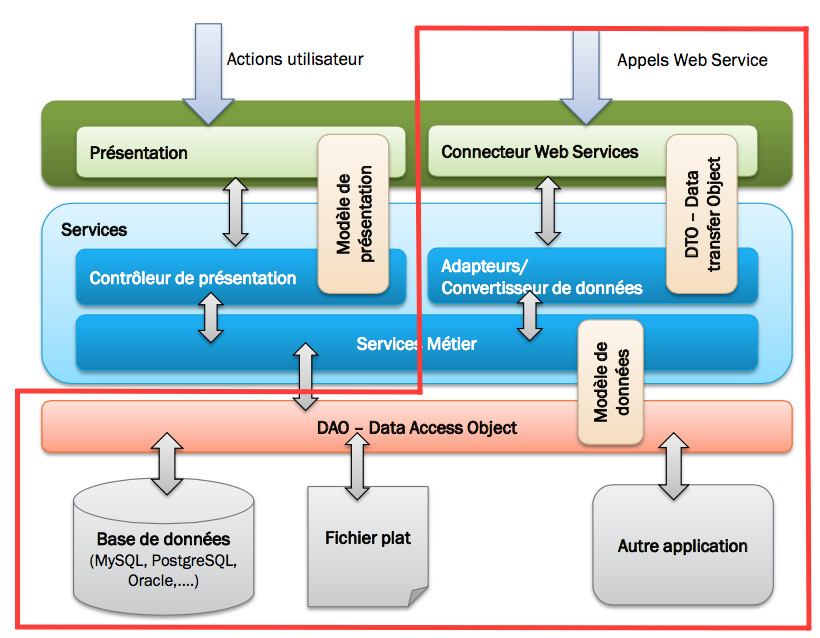
\includegraphics[scale=0.3]{images/WebAppArchitecture2.png}
\end{figure}
\end{block}
\end{frame}
\subsection{Livrables attendus}
\begin{frame}{Livrables attendus}
\begin{block}{Livrables}
\begin{itemize}
\item Un module maven s'intégrant au projet parent
\item Un web service en mode asynchrone
\item Un service dédié GTFS fonctionnel
\item Des classes abstraites pour la généricité du service
\end{itemize}
\end{block}
\end{frame}

\AtBeginSection[]
{
  \begin{frame}<beamer>
\begin{multicols}{2}
     \tableofcontents[currentsection,hideothersubsection]
   \end{multicols}
  \end{frame}
}

\section{Gestion de projet}
\subsection{Planning et suivi }
\begin{frame}{Planning et suivi / Environnement humain }
\begin{block}{Planning et suivi}
Un point de suivi informel plusieurs fois par semaine :\\
	- présentation du travail effectué, \\
	- des résultats intermédiaires,\\ 
	- planifier la semaine à venir\\
	
Un bilan à la mi-stage a été effectué afin de réajuster les priorités
\end{block}
\begin{block}{Environnement humain}
	Travail dans un \og Open space \fg, avec une dizaine de collaborateurs, à côté du chef de projet \og MobiSAAS \fg{} 
\end{block}
\end{frame}
\subsection{Environnement technique}
\begin{frame}{Environnement technique}
\begin{block}{Environnement technique}
	Environnement MS Windows (lié aux technologies ESRI),\\
	
	SGDB Postgresql, lié à l'utilisation dans quasi tous les projets de l'extension spatiale Postgis.\\
	
	2 IDE : Liclipse (Python) et Eclipse (Java)\\
	
\end{block}
\begin{block}{Technologies Java remarquables }
\begin{itemize}
\item Apache Maven
\item Framework \og Dropwizard \fg
\item Hibernate
\item Jackson
\end{itemize} 
\end{block}
\end{frame}
\subsection{Objectifs de qualité}
\begin{frame}{Objectifs de qualité}
\begin{block}{Objectifs de qualité}
\begin{itemize}
\item Adaptabilité = abstraction
\item Testabilité = nombreux tests et jeux de données pour tester
\item Fiabilité = outil fonctionnel
\item Sécurité = intégrité des données, accès aux services avec authentification
\end{itemize}
\end{block}
\end{frame}

\AtBeginSection[]
{
  \begin{frame}<beamer>
\begin{multicols}{2}
     \tableofcontents[currentsection,hideothersubsection]
   \end{multicols}
	\end{frame}
}

\section{Analyse / Conception}
\subsection{Analyse}
\begin{frame}{Analyse}
\begin{block}{Organisation du projet}
\begin{figure}[h]
    \center
    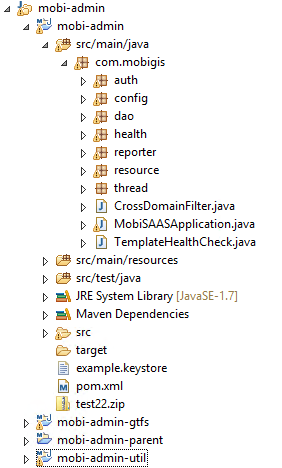
\includegraphics[scale=0.6]{images/Package_explorer_MobiSAAS.PNG}
\end{figure}
\end{block}
\end{frame}
\begin{frame}{Analyse}
\begin{block}{Organisation du module \og mobi-admin-gtfs \fg}

\begin{figure}[h]
\begin{columns}[c]
    \column{.005\textwidth}
       \begin{flushleft}
	   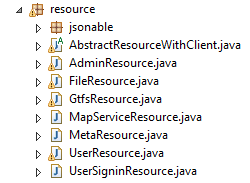
\includegraphics[scale=0.5]{images/Package_explorer_MobiSAAS_Resource.PNG}
		\end{flushleft}
    \column{.005\texwidth}
       \begin{flushleft}    
    	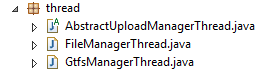
\includegraphics[scale=0.5]{images/Package_explorer_MobiSAAS_Thread.PNG}
       \end{flushleft}
\end{columns}
\end{figure}
\end{block}
\end{frame}
\begin{frame}{Analyse}
\begin{block}{Approche générique}
\begin{figure}[h]
    \center
    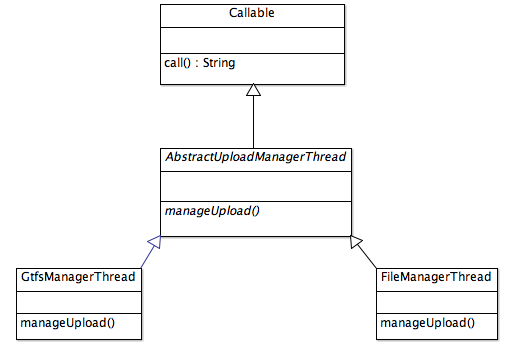
\includegraphics[scale=0.5]{images/DiagrammeThread.png}
\end{figure}
\end{block}
\end{frame}
\subsection{Conception}
\begin{frame}{Conception}
\begin{block}{Réalisations}
\begin{itemize}
\item Documentation de l'API
\item Schéma de conception UML
\item Modèle de base de données
\item Jeux de données tests / suite de tests (SOAP UI)
\item Plan de charge (cf. perspectives)
\end{itemize}
\end{block}
\end{frame}
\AtBeginSection[]
{
  \begin{frame}<beamer>
  \begin{multicols}{2}
     \tableofcontents[currentsection,hideothersubsection]
   \end{multicols}
	\end{frame}
}

\section{Codage}
\subsection{Bonnes pratiques}
\begin{frame}{Bonnes pratiques}
\begin{block}{Exemples}
	Javadoc\\
	Commentaires\\
	Logging\\
	Discussions quotidiennes\\
	Approche RESTFul (verbe, pluriels,...)\\
	Tests\\
\end{block}
\end{frame}
\subsection{Codage}
\begin{frame}{Codage}
\begin{block}{Eléments remarquables du code}
Domaine métier : \\
\item POJO 
\item DAO
\item Service\\

Programmation concurrente :\\
 \textrightarrow  	framework Executor (Callable)
\end{block}
\end{frame}

\AtBeginSection[]
{
  \begin{frame}<beamer>
  \begin{multicols}{2}
     \tableofcontents[currentsection, hideothersubsection]
   \end{multicols}
  \end{frame}
}

\section{Présentation des éléments les plus significatifs de l'interface de l'application}
\subsection{Résultats}
\begin{frame}{Résultats}
\begin{block}{Résultats terminés}
GtfsResource() : GET (1), GET (ALL), POST, DELETE\\

FileResource() : GET (1), GET (ALL), POST, DELETE\\

AbstractUploadManagerThread() : Généricité, mode asynchrone, programmation concurrente
\end{block}
\begin{block}{Résultats en cours}
\begin{itemize}
\item LoadData() : csv to postgresql = à finaliser, à mettre en resource (Web Service)
\end{itemize}
\end{block}
\begin{block}{Perspectives}
Exploiter la librairie OneBusAway :
\begin{itemize}
\item MergeData() : fusionner 2 sources
\item RetainData() : permettre sélection : routes, dates,…
\end{itemize}
Continuer la prise en main de Dropwizard et des données
\end{block}
\end{frame}
\AtBeginSection[]
{
  \begin{frame}<beamer>
\begin{multicols}{2}
     \tableofcontents[currentsection,hideothersubsection]
   \end{multicols}
	\end{frame}
}
\section{Synthèse et conclusion}
\subsection{Bilan professionnel}
\begin{frame}{Bilan professionnel}
\begin{block}{Bilan professionnel}
J'ai pu intégrer un projet innovant me permettant de découvrir énormément de choses : REST, Dropwizard, JSON, etc.\\

Cette expérience est pour moi très valorisante tant d'un point de vue humain que technique, elle répond parfaitement à mes attentes.\\

~\\
De plus, la mise en pratique de mes connaissances théoriques en Java se sont parfaitement concrétisées au domaine d'application des Systèmes d'Information Géographique (SIG) dans lequel j'exerçais auparavant en tant que Géomaticien.
\end{block}
\end{frame}
\subsection{Bilan personnel}
\begin{frame}{Bilan personnel}
\begin{block}{Bilan personnel}
J'ai découvert un nouveau domaine en plein développement et propice à l'innovation, celui des \og Transports\fg \\
~\\

Ce stage a été pour moi l'occasion de pratiquer des langages tels que Python ou Java, langages largement répandus dans le monde industriel.\\
~\\

J'ai aussi réalisé mon mémoire et cette présentation avec le langage  \LaTeX{}.
\end{block}
\end{frame}


% Dernière slide de Conclusion
\subsection{Conclusion}
\begin{frame}{Conclusion}
\begin{block}{Conclusion}
Mon intégration à l'équipe technique, et aux projets ? 
~\\
\textrightarrow  	CDD de 6 mois

~\\
~\\

Cette expérience d'un point de vue académique ?
~\\
\textrightarrow 	12 compétences sur les 15 nécessaires à l'obtention du titre ont été abordées. 
\end{block}
\end{frame}

\begin{frame}{Fin}
\centering
\textbf{Merci de votre attention}

\end{frame}


\end{document}

